% $HeadURL: https://sbgn.svn.sourceforge.net/svnroot/sbgn/trunk/documents/specifications/EntityRelationship/Level1/sources/transition.tex $

%%%%%%%%%%%%%%%%%%%%%%%%%%%%%%%%%%%%%%%%%%%%%%%%%%%%%%%%%%%%%%%%%%%%%%
%%                     Transition
%%%%%%%%%%%%%%%%%%%%%%%%%%%%%%%%%%%%%%%%%%%%%%%%%%%%%%%%%%%%%%%%%%%%%%
\color{red}
\subsection{Glyph: \glyph{Transition}}
\label{sec:transition}

A transition is a process transforming a set of entities (represented by \glyph{ENs} in \SBGNPDLone) into another set entities.

\begin{glyphDescription}

\glyphSboTerm SBO:0000167 ! reaction

\glyphOrigin One or several \glyph{consumption} arcs (\sect{consumption}) or one or several \glyph{production} arcs (\sect{production}).

\glyphTarget One or several \glyph{production} arcs (\sect{production}).

\glyphNode A transition is represented by a square box linked to two connectors, small arcs attached to the centers of opposite sides. The consumption (\sect{consumption}) and production (\sect{production}) arcs are linked to the extremities of those connectors. The modulatory arcs (\sect{arcs}) point to the other two sides of the box. A \glyph{transition} connected to \glyph{production} arcs on opposite sides is a reversible transition. The connectors and the box move as a rigid entity.

\end{glyphDescription}

\begin{figure}[H]
  \centering
  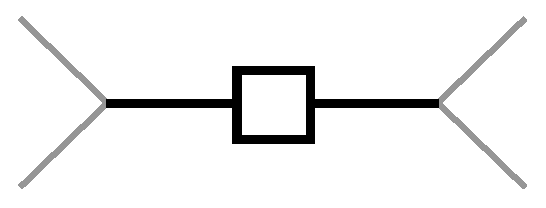
\includegraphics[scale = 0.4]{images/transition}
  \caption{The \ER glyph for \glyph{transition}.}
  \label{fig:transition}
\end{figure}

A transition is the basic process node in SBGN.  It describes a process that transforms a given set of biochemical entities---macromolecules, simple chemicals or unspecified entities---into another set of biochemical entities.  Such a transformation might imply modification of covalent bonds (conversion), modification of the relative position of constituents (conformational transition) or movement from one compartment to another (translocation).

A cardinality label may be associated with \glyph{consumption} (\sect{consumption}) or \glyph{production} (\sect{production}) arcs to indicate the stoichiometry of the process.  This label becomes a requirement when the exact composition of the number of copies of the inputs or outputs to a reaction are ambiguous in the diagram.

The example in \fig{trans-react} illustrates the use of a \glyph{transition} node to represent a reaction between two reactants that generates three products. 

\begin{figure}[H]
  \centering
  \includegraphics[scale = 0.3]{examples/transition-reaction}
  \caption{A reaction that generates three products.}
  \label{fig:trans-react}
\end{figure}
 
% SHOULD BECOME AN ASSIGNMENT
%
% The example in \fig{trans-trans} illustrates the use of a \glyph{transition} node to represent a translocation. The large round-cornered rectangle represents a compartment border (see \sect{compartment}).
% 
% \begin{figure}[H]
%   \centering
%   \includegraphics[scale = 0.3]{examples/transition-translocation}
%   \caption{A translocation.}
%   \label{fig:trans-trans}
% \end{figure}

\normalcolor

% The following is for [X]Emacs users.  Please leave in place.
% Local Variables:
% TeX-master: "../sbgn_ER-level1"
% End:
